\begin{frame}{Équations d'ADR}{Stratégies de simulation}
    \textbf{Stratégie $n^o1$ : Différencier le traitement sur chaque opérateurs}\\
        Ne pas faire un schéma monolithique.
        \begin{itemize}
            \item Séparation d'opérateurs (\emph{splitting})
            \item Méthodes ImEx (Additive Runge et Kutta)
        \end{itemize}
        \pause
\noindent\color{Primary}\rule{\linewidth}{0.6pt}\color{black}

    \textbf{Stratégie $n^o2$ : Adaptation en espace}\\
        La multirésolution adaptative : 
        \begin{itemize}
            \item Des grilles de \emph{résolution multiples},
            \item Deux opérateurs de \emph{projection/reconstruction},
            \item Représentation de la solution comme une suite de \emph{détails},
            \item Une stratégie d'\emph{adaptation}.
        \end{itemize}
    \color{red}    \centering
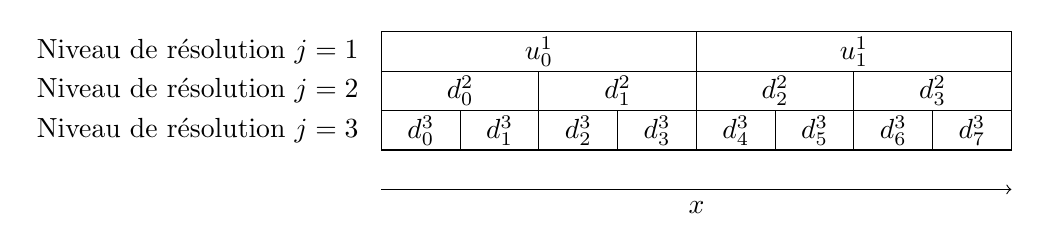
\begin{tikzpicture}


\node[anchor=west] at (-8.5, -.25) {Niveau de résolution $j=3$};
\node[anchor=west] at (-8.5, .25) {Niveau de résolution $j=2$};
\node[anchor=west] at (-8.5, .75) {Niveau de résolution $j=1$};
% Niveau j-1
\draw[->] (-4,-1) -- (4,-1);
\draw (-4,.5) rectangle (0,1);
\draw (0,.5) rectangle (4,1);
\node[anchor=center] at (0, -1.23) {$x$};

    % Niveau j
\draw (-4,0) rectangle (-2,.5);
\draw (-2,0) rectangle (0,.5);
\draw (0,0) rectangle (2,.5);
\draw (2,0) rectangle (4,.5);
%\node at (1,1.75) {$k=2$};

% Niveau j+1

\draw (-4,-.5) rectangle (-3,0);
\draw (-3,-.5) rectangle (-2,0);
\draw (-2,-.5) rectangle (-1,0);
\draw (-1,-.5) rectangle (0,0);
\draw (0,-.5) rectangle (1,0);
\draw (1,-.5) rectangle (2,0);
\draw (2,-.5) rectangle (3,0);
\draw (3,-.5) rectangle (4,0);

% Relations
\node at (-2, .75) {$u^1_0$};
\node at (+2, .75) {$u^1_1$};

\node at (-3, .25) {$d^2_0$};
\node at (-1, .25) {$d^2_1$};
\node at (+1, .25) {$d^2_2$};
\node at (+3, .25) {$d^2_3$};

\node at (-3.5, -.25) {$d^3_0$};
\node at (-2.5, -.25) {$d^3_1$};
\node at (-1.5, -.25) {$d^3_2$};
\node at (-0.5, -.25) {$d^3_3$};

\node at (+0.5, -.25) {$d^3_4$};
\node at (+1.5, -.25) {$d^3_5$};
\node at (+2.5, -.25) {$d^3_6$};
\node at (+3.5, -.25) {$d^3_7$};


\end{tikzpicture}

\end{frame}